\section{Parametervariation}
\label{sec:wellen:parametervariation}

Die Anfangsbedingungen $a_0$ und $a_1$ k"onnen beliebig festgelegt werden. Da 
sich die Wellen im betrachteten Fall um den Entwicklungspunkt $x_0=0$ bewegen, 
beschreibt das $a_0$ den y-Achsenabschnitt und das $a_1$ die Steigung im Punkt 
$y(0)$.

\subsection{Bedeutung von \texorpdfstring{$a$}{a}, \texorpdfstring{$b$}{b} und 
\texorpdfstring{$c$}{c}}
Die drei Parameter $a$, $b$ und $c$ haben jeweils unterschiedliche Auswirkungen 
auf die Parabel. So kann mit $a$ der Schnittpunkt mit der $x$-Achse und mit $c$ 
derjenige mit der $y$-Achse festgelegt werden. $b$ hingegen verschiebt die 
ganze Parabel in verschiedene Richtungen. Da diese Eigenschaft f"ur das 
gegebene Modell nicht relevant ist, wird grunds"atzlich
\begin{equation*}
	b = 0
\end{equation*}
gesetzt.

\subsection{Lineare Differentialgleichung}
\label{subsec:wellen:linearedifferntialgleichung}

Indem $a$ verschwindend klein gew"ahlt wird, entsteht
\begin{equation}
	y''+ cy = 0.
	\label{eq:wellen:lineareDGL}
\end{equation}

Diese lineare Differentialgleichung kann mit Hilfe des charakteristischen 
Polynoms
\begin{equation*}
	p(\lambda) = [(\lambda+\mu)^2+\omega^2] = 0
\end{equation*}
dessen L"osungen
\begin{equation*}
\begin{split}
	y_1 &= C_1e^{-\mu x}\cos(\omega x) \\
	y_2 &= C_2e^{-\mu x}\sin(\omega x)
\end{split}
\end{equation*}
sind, gel"ost werden.

Angewandt auf die Gleichung \ref{eq:wellen:lineareDGL} ergibt sich nun zu
\begin{equation*}
\begin{split}
	p(\lambda) &= [(\lambda+0)^2+\sqrt{c}^2] = 0 \\
	\Leftrightarrow p(\lambda) &= [\lambda^2+c] = 0,
\end{split}
\end{equation*}
was uns nun
\begin{equation}
y(x) = C_1 \cos(\sqrt{c}x) + C_2 \sin(\sqrt{c}x)
\label{eq:wellen:loesunglinearedgl}
\end{equation}
als L"osung ergibt.

Um die Konstanten $C_1$ und $C_2$ zu bestimmen m"ussen die Anfangsbedingungen 
$a_0$ und $a_1$ bekannt sein. Damit die Abh"angigkeit auf gezeigt werden kann, 
wird zuerst die erste Ableitung der L"osung \ref{eq:wellen:loesunglinearedgl} 
aufgestellt werden.

\begin{equation}
	y'(x)=-C_1 \sqrt{c} \sin(\sqrt{c}x) + C_2 \sqrt{c} \cos(\sqrt{c}x)
\end{equation}

Die Werte von $y(0)$ und $y'(0)$ sind jeweils durch $a_0$ beziehungsweise $a_1$ 
gegeben. Setzt man nun $x = 0$ ein, ergibt sich f"ur $C_1$ und $C_2$
\begin{equation}
	\begin{split}
		y(0) = C_1 = a_0 &\Leftrightarrow C_1 = a_0 \\
		y'(0) = C_2 \sqrt{c} = a_1 &\Leftrightarrow C_2 = \frac{a_1}{\sqrt{c}}.
	\end{split}
\end{equation}

Eingesetzt in \ref{eq:wellen:loesunglinearedgl} erhalten wir nun
\begin{equation*}
	y(x) = a_0 \cos(\sqrt{c}x) + \frac{a_1}{\sqrt{c}} \sin(\sqrt{c}x), \qquad c 
	> 0
\end{equation*}
und
\begin{equation}
\begin{split}
	y(x) &= a_0 \cos(i\sqrt{|c|}x) + \frac{a_1}{i\sqrt{|c|}}\sin(i\sqrt{|c|}x), 
	\qquad c < 0\\
	\Leftrightarrow
	y(x) &= a_0 \cos(i\sqrt{|c|}x) - i\frac{a_1}{\sqrt{|c|}}\sin(i\sqrt{|c|}x)\\
	\Leftrightarrow
	y(x) &= a_0 \cosh(\sqrt{|c|}x) + \frac{a_1}{\sqrt{|c|}}\sinh(\sqrt{|c|}x).
\end{split}	
\end{equation}
Der letzte Umformungsschritt ergibt sich aus der Definition von $\cosh$ und 
$\sinh$:
\begin{equation*}
\begin{split}
	\sinh(x) &= \frac{1}{2} (e^x - e^{-x}) = -i \sin(ix)\\
	\cosh(x) &= \frac{1}{2} (e^x + e^{-x}) = \cos (ix)
\end{split}
\end{equation*}

Die gefundenen L"osungen k"onnen auch graphisch best"atigt werden. Sei es f"ur 
positve $c$ in Form von $\sin$ und $\cos$:

\noindent
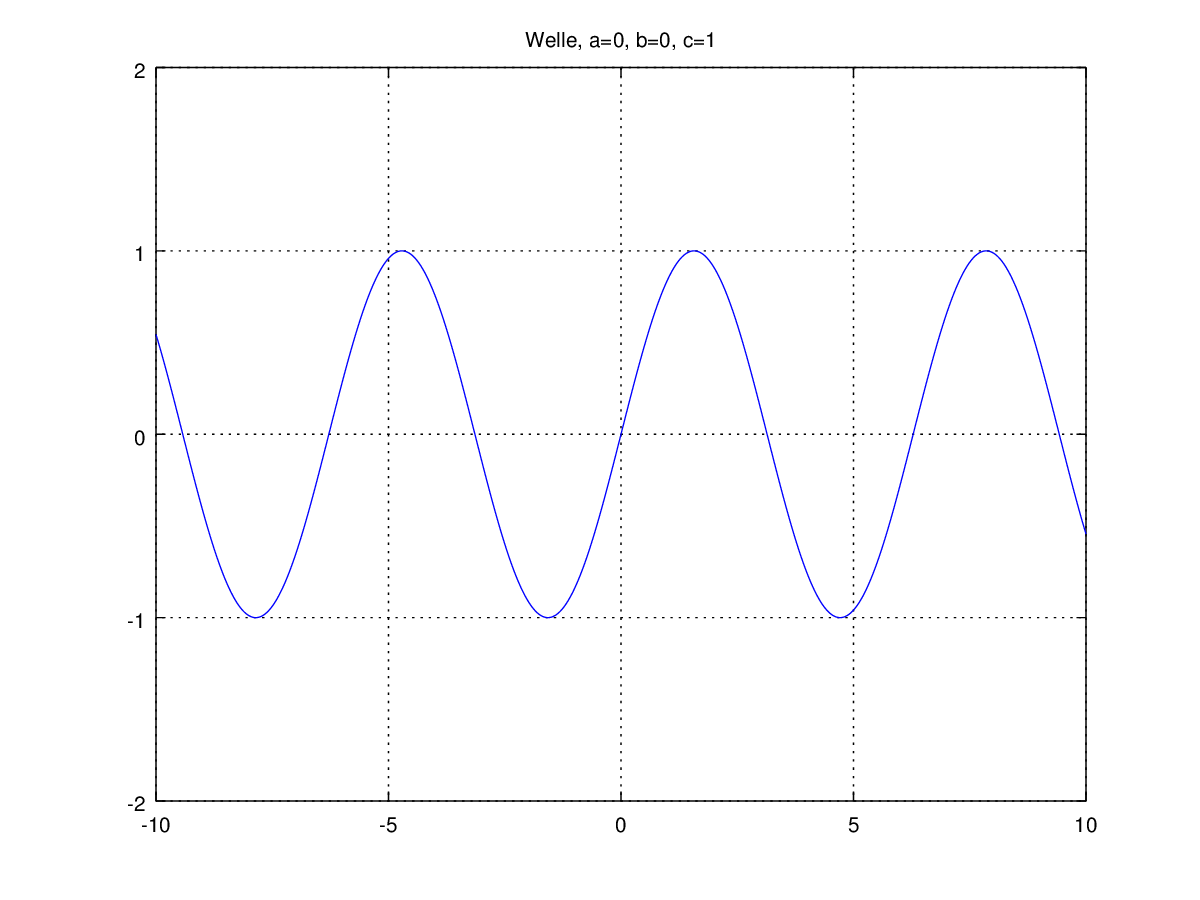
\includegraphics[scale=0.35]{./wellen/images/basicfunctions/sin.png}
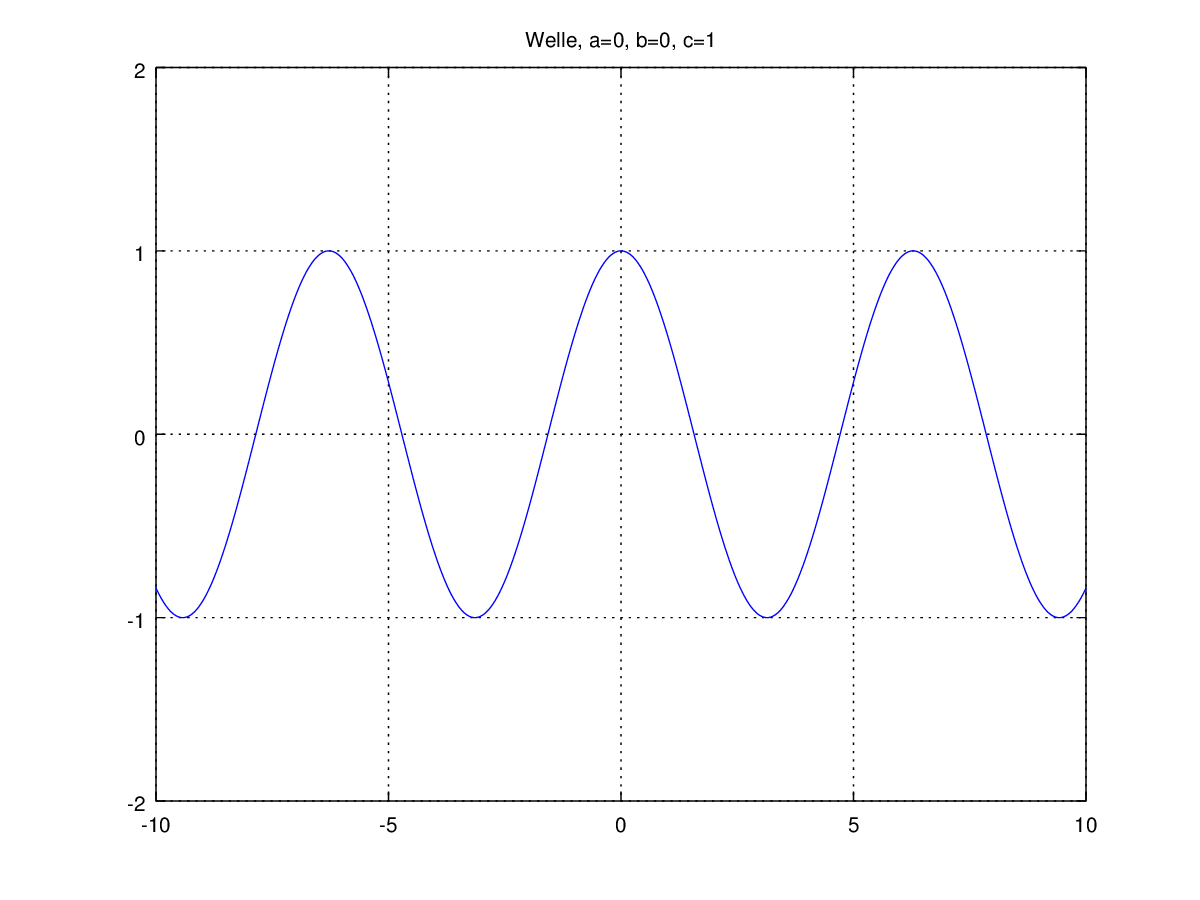
\includegraphics[scale=0.35]{./wellen/images/basicfunctions/cos.png}

oder $\sinh$ und $\cosh$ f"ur negative $c$:

\noindent
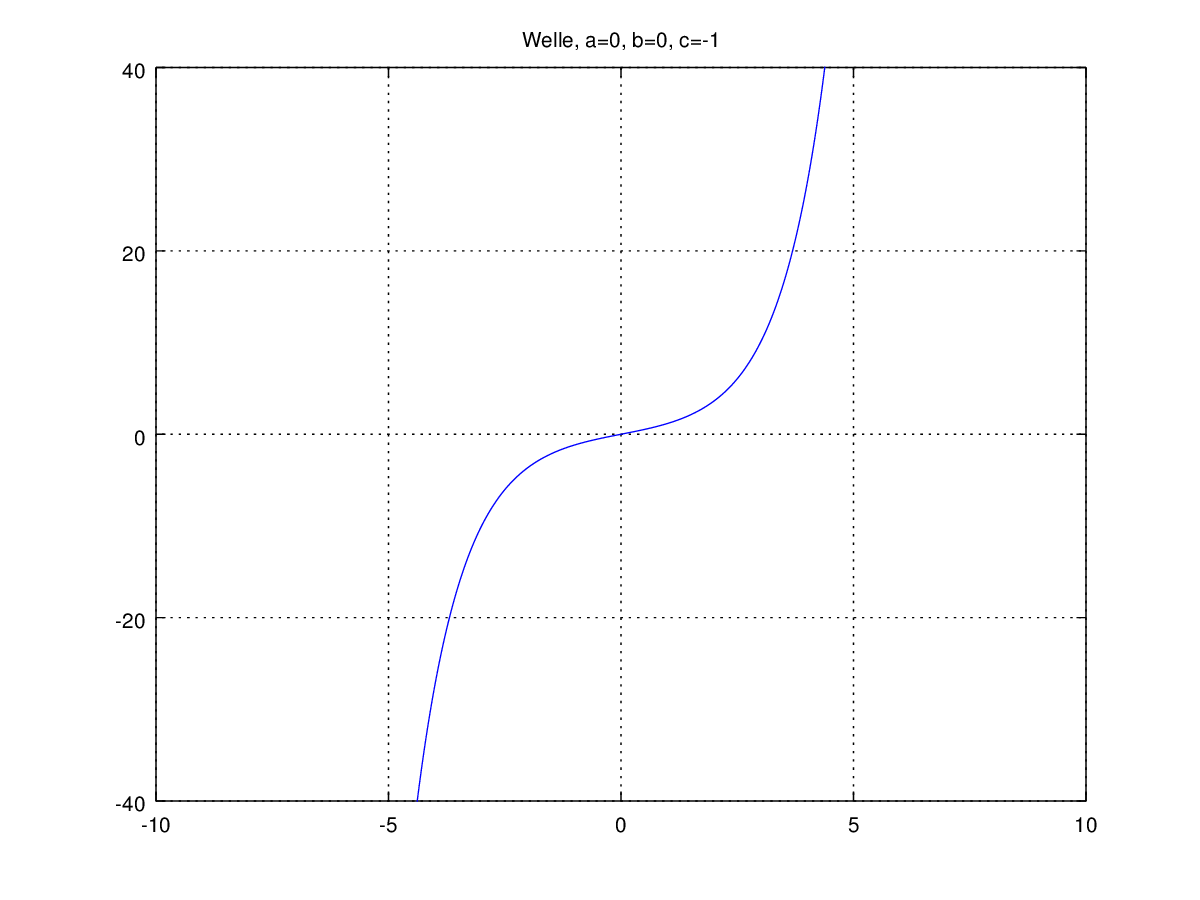
\includegraphics[scale=0.35]{./wellen/images/basicfunctions/sinh.png}
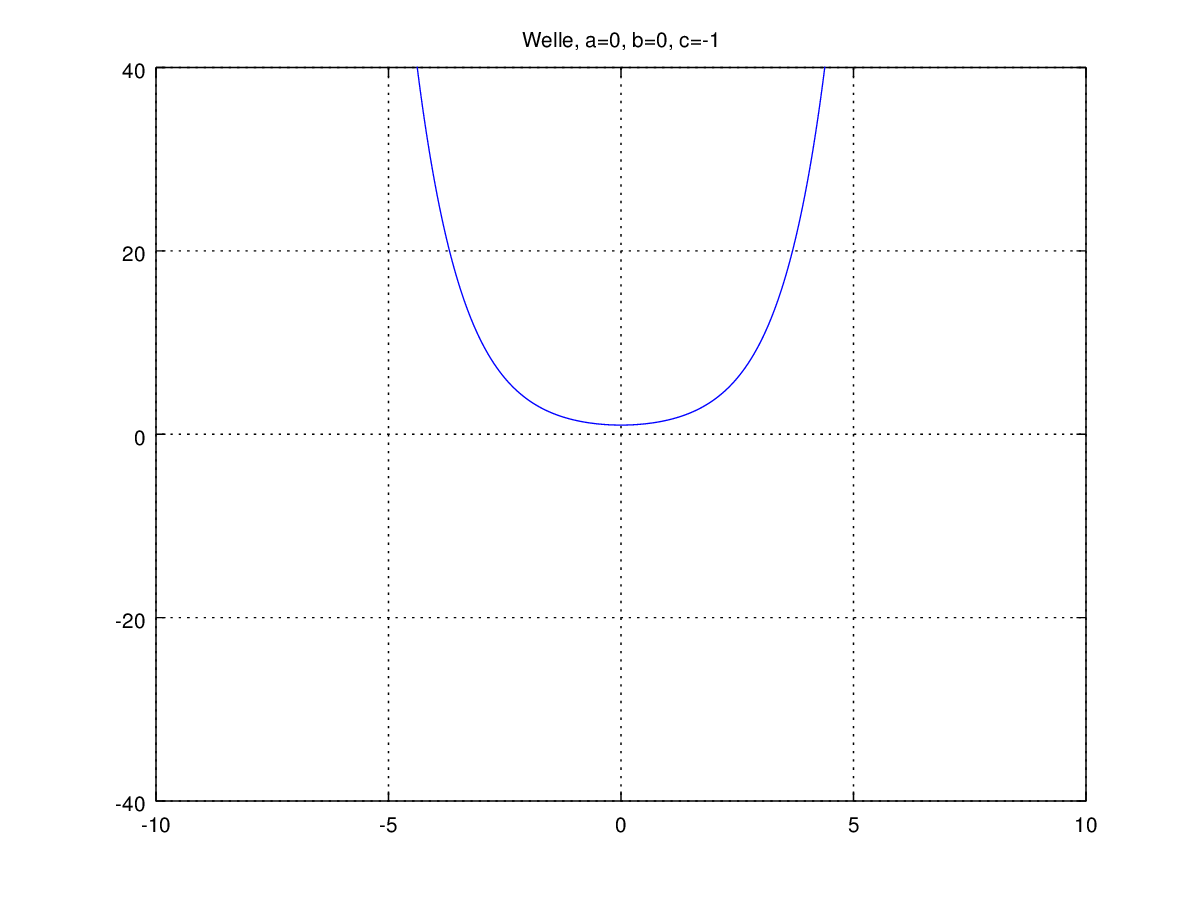
\includegraphics[scale=0.35]{./wellen/images/basicfunctions/cosh.png}

\subsection{Parabelformen}
\label{subsec:wellen:parabelformen}

Wenn nur $c$ angepasst wird erhalten wir:

\noindent
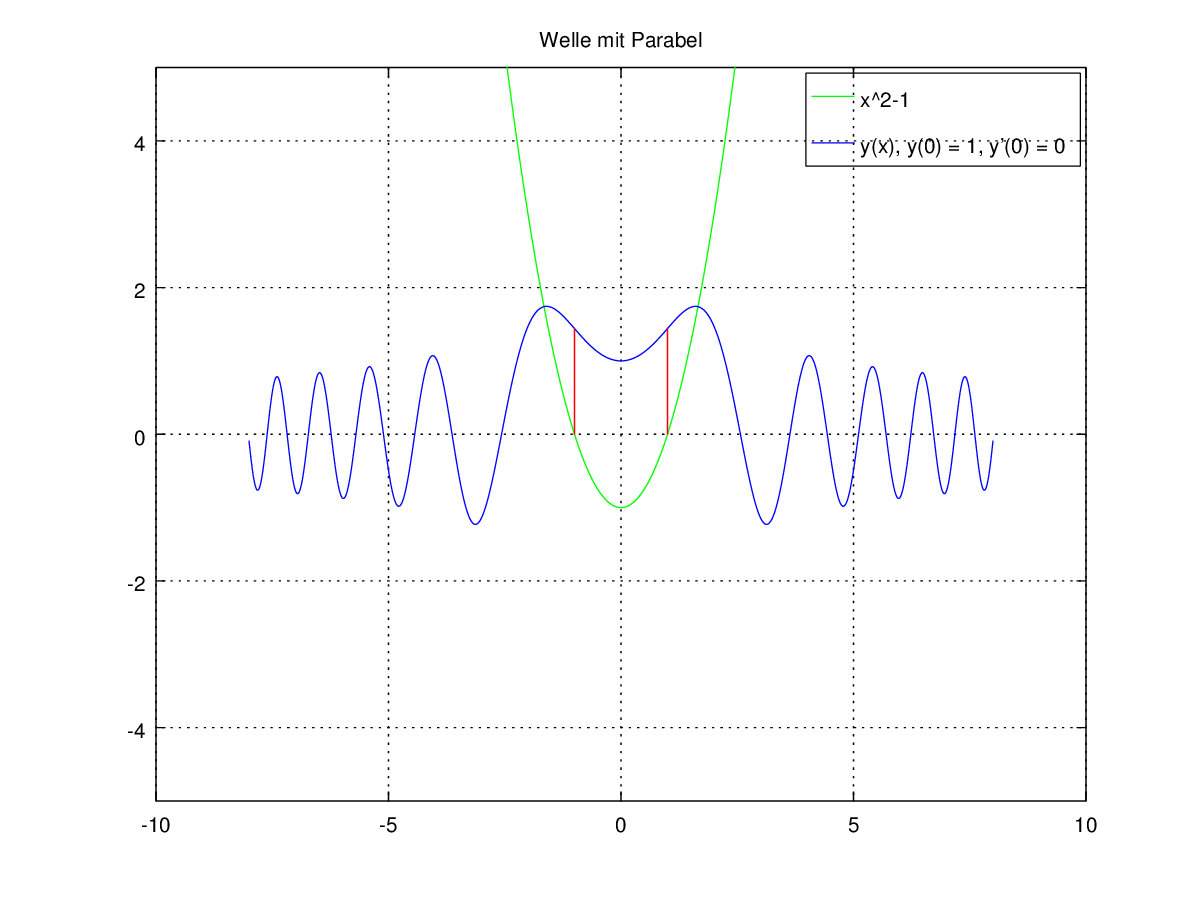
\includegraphics[scale=0.35]{./wellen/images/varc/cneg1.png}
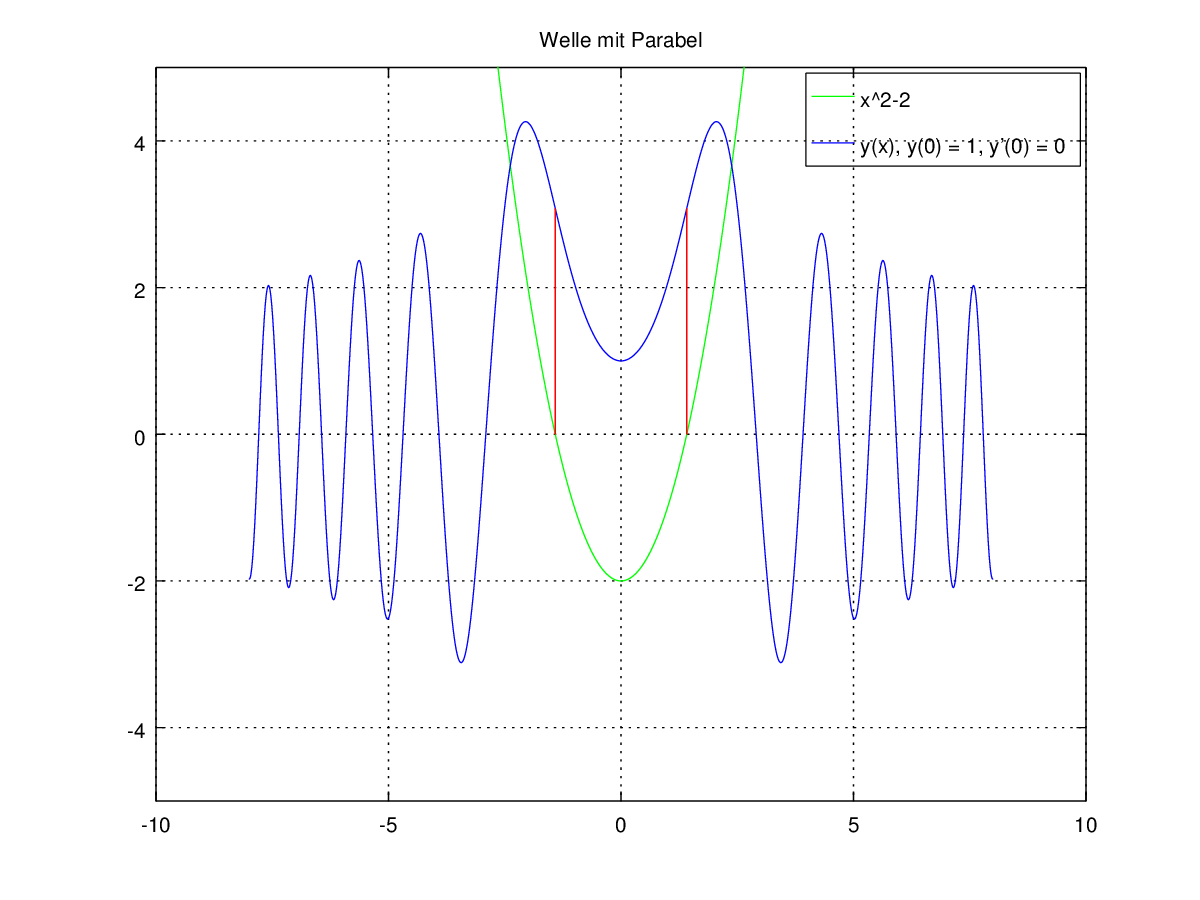
\includegraphics[scale=0.35]{./wellen/images/varc/cneg2.png}

Wenn nur $a$ angepasst wird erhalten wir:

\noindent
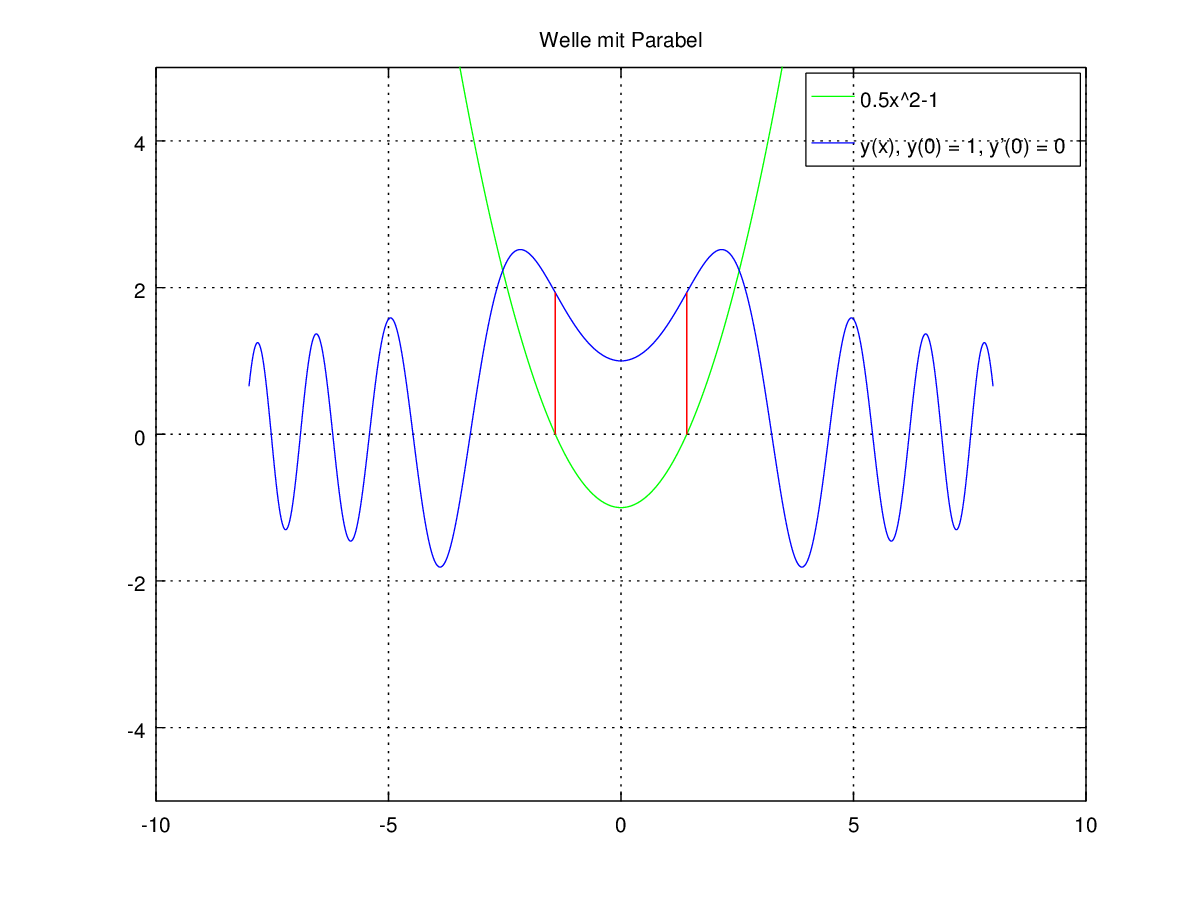
\includegraphics[scale=0.35]{./wellen/images/vara/ahalbe.png}
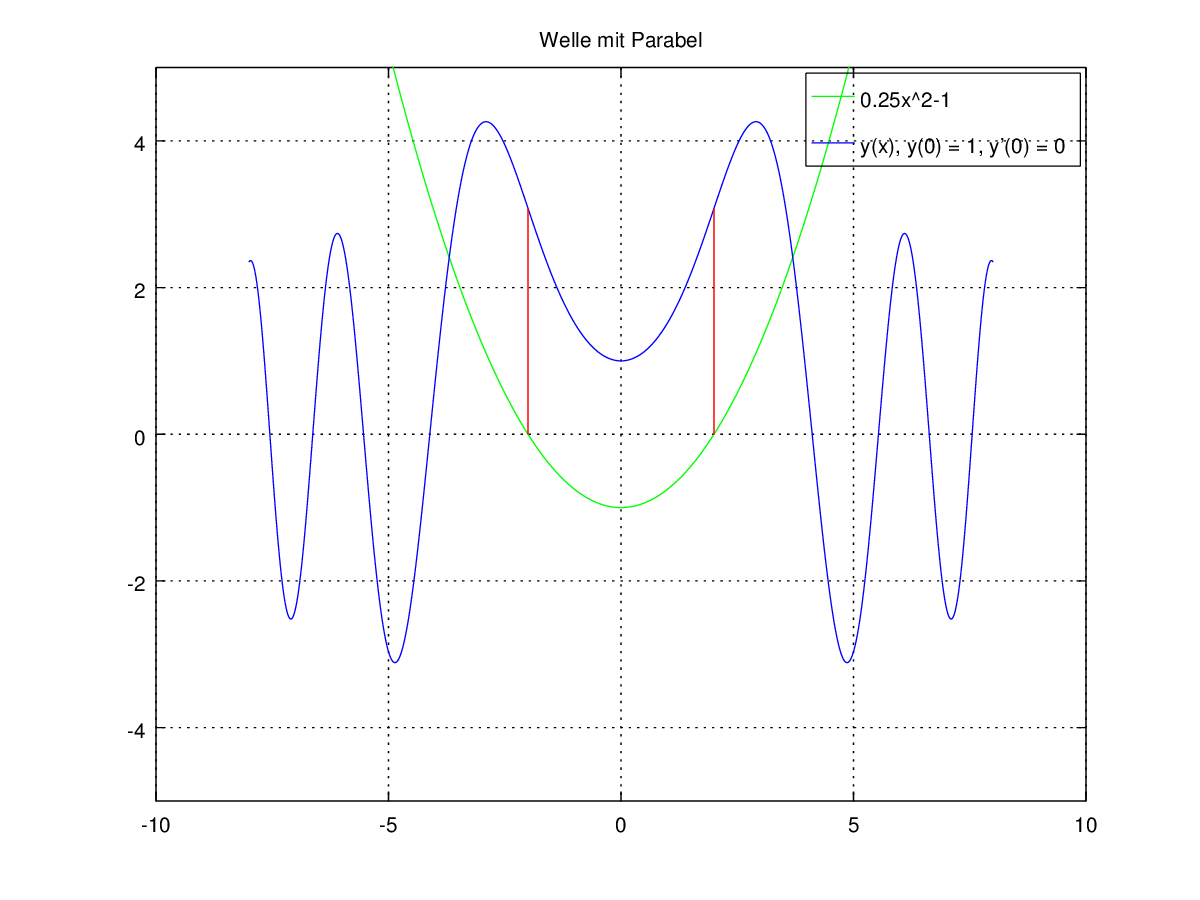
\includegraphics[scale=0.35]{./wellen/images/vara/aviertel.png}

Obwohl die Wellenformen alle "ahnlich sind, stellen wir fest, dass es bei den 
jeweiligen Nullstellen der Parabel eine gr"ossere Ver"anderung gibt.
